\documentclass[a4paper, 11pt]{article}
\usepackage{geometry}
\usepackage{indentfirst}
\usepackage{setspace}
\usepackage{amsmath}
\usepackage{graphicx}
\usepackage{wrapfig}
\usepackage{caption}
\usepackage{indentfirst}
\usepackage{amssymb}
\usepackage{float}


\graphicspath{ {./images/} }
\geometry{left=2.5cm, right=2.5cm, top=2.5cm, bottom=3cm}

\begin{document}
	% Upload all the source files and a report containing:
	% Answer to theoretical questions,
	% a brief description of the methods,
	% some comments to the results
	% all the outputs.
	
	\title{Exercise \# 1. Numerical methods for ODES. }
	\author{{\small Alexandre Rodrigues (2039952)}}
	\date{\today}
	
	\maketitle
	
	\section*{Intro}
	%
	
	\section*{Methods}
	% Brief description of the methods
	
	
	\section*{Answers}
	% answer to theoretical questions
	\subsection*{Question 1}
	
	\begin{equation}
		y(t) = e^{-5t}
	\end{equation}
	
	\begin{figure}[H]
		\centering
		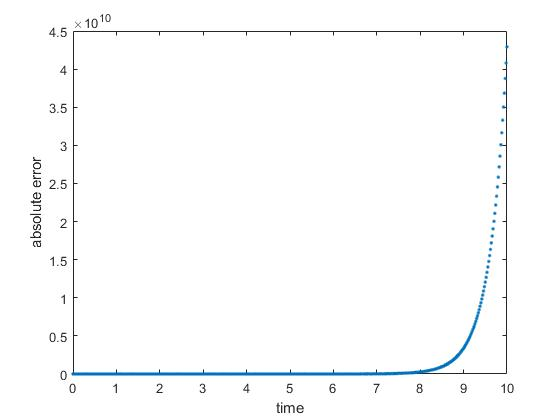
\includegraphics[width=\linewidth]{ex1_fe.jpg}
		\caption{Absolute error in function of time using Forward Euler method to compute y(1)}
		\label{fig:ex1_fe}
	\end{figure}
	
	We got a maximum error of $4.2916 \times 10^{10}$...
	
	\begin{figure}[H]
		\centering
		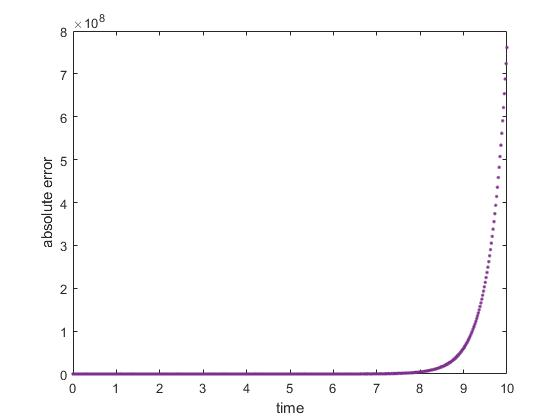
\includegraphics[width=\linewidth]{ex1_rk4.jpg}
		\caption{Absolute error in function of time using RK4 method to compute y(1)}
		\label{fig:ex1_rk4}
	\end{figure}
	
	We got a maximum error of $4.3146 \times 10^{10}$...
	
	%d)
	\subsubsection*{Comment the different behavior observed by the numerical method.}
		The Simpson's method has an empty stability region as proved by: $\ldots$
		We can notice the difference in the initial conditions in our results.
		The FE calculation for y(2) is better then the RK4 calculation given the best final error.
		This is, although, not that relevant, the difference is of about $ 0.5 \times 10^{-10} \% $.
%		We can conclude that, due to the clear instability of the Simpson's method, the initial conditions 
	
	\subsection*{Question 2}
	
	The exact solution can be found as:
	\begin{equation}
		y(t) = \frac{1}{10t + 1}
	\end{equation}
	
	\begin{figure}[H]
		\centering
		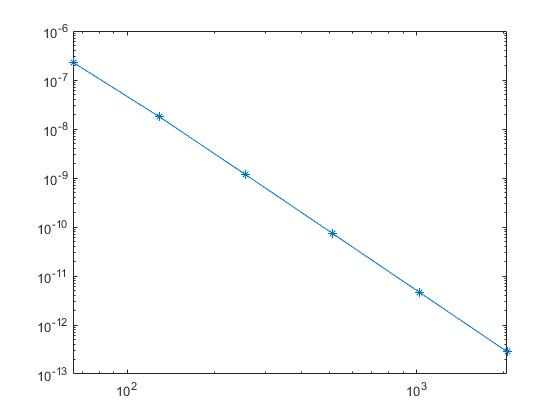
\includegraphics[width=\linewidth]{ex2.jpg}
		\caption{LogLog plot of the error as a function of the number of steps.}
		\label{fig:ex2}
	\end{figure}
	
	\begin{table}[H]
		\centering
		\begin{tabular}{c|c}
			\textbf{$h$}& \textbf{error}   \\ \hline
			$ 3.125000\times 10^{-2} $ & $ 2.291844\times 10^{-7} $ \\ \hline
			$ 1.562500\times 10^{-2} $ & $ 1.785763\times 10^{-8} $ \\ \hline
			$ 7.812500\times 10^{-3} $ & $ 1.160234\times 10^{-9} $ \\ \hline
			$ 3.906250\times 10^{-3} $ & $ 7.312862\times 10^{-11} $ \\ \hline
			$ 1.953125\times 10^{-3} $ & $ 4.579586\times 10^{-12} $ \\ \hline
			$ 9.765625\times 10^{-4} $ & $ 2.863750\times 10^{-13} $ \\ \hline
		\end{tabular}
	\end{table}
	
	The error reduces with the increase in the number of steps due to the decrease of $h$ as expected in theory. $\ldots$		
	
	\subsection*{Question 3}
	% Nothing done....
	
	\subsection*{Question 4}
	%....
	%a) stabilty? how?
	%b) Nothing done....
	%c) Nothing done....
	
	\subsection*{Question 5}
	\begin{figure}[H]
		\centering
		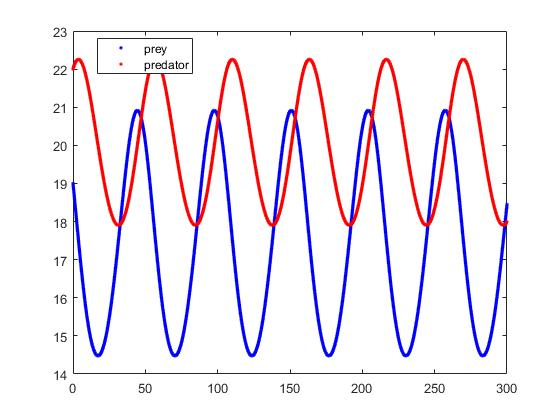
\includegraphics[width=\linewidth]{ex5.jpg}
		\caption{Evolution of the number of preys and predators.}
		\label{fig:ex5}
	\end{figure}
	
	
	
	
	
	\section*{Results}
	% comments to the results
	
	
	\section*{Outputs}
	
	
	
\end{document}



